\let\negmedspace\undefined
\let\negthickspace\undefined
\documentclass[12pt]{article}
\usepackage{cite}
\usepackage{float}
\usepackage{amsmath,amssymb,amsfonts,amsthm}
\usepackage{algorithmic}
\usepackage{graphicx}
\usepackage{textcomp}
\usepackage{xcolor}
\usepackage{txfonts}
\usepackage{listings}
\usepackage{enumitem}
\usepackage{mathtools}
\usepackage{gensymb}
\usepackage{comment}
\usepackage[breaklinks=true]{hyperref}
\usepackage{tkz-euclide} 
\usepackage{listings}
\usepackage{gvv}                                                             
\usepackage{gvv-book}     
\usepackage{xparse}
\usepackage{color}                                            
\usepackage{array}                                            
\usepackage{longtable}                                       
\usepackage{calc}                                             
\usepackage{multirow}
\usepackage{multicol}
\usepackage{hhline}                                           
\usepackage{ifthen}                                           
\usepackage{lscape}
\usepackage{tabularx}
\usepackage{array}
\usepackage{float}
\usepackage{geometry}

\geometry{left=1in, right=1in, top=1in, bottom=1in}

\begin{document}

\begin{center}
    \Large \textbf{GATE 2022 Biotechnology (BT)}
\end{center}

\section*{General Aptitude}

\section*{Q.1 -- Q.5 carry one mark each.}

\begin{enumerate}[leftmargin=2.5em, label=\textbf{Q.\arabic*}., itemsep=2em]

\item You should \_\_\_\_\_\_\_ when to say \_\_\_\_\_\_\_.

\noindent \textbf{[GATE BT 2022]}
\begin{multicols}{2}
\begin{enumerate}
    \item no / no
    \item no / know
    \item know / know
    \item know / no
\end{enumerate}
\end{multicols}

\item Two straight lines pass through the origin $(x,y) = (0,0)$. One of them passes through the point $(1,3)$ and the other passes through the point $(1,2)$.  
What is the area enclosed between the straight lines in the interval $[0,1]$ on the $x$-axis?

\noindent \textbf{[GATE BT 2022]}
\begin{multicols}{2}
\begin{enumerate}
    \item 0.5
    \item 1.0
    \item 1.5
    \item 2.0
\end{enumerate}
\end{multicols}

\item If
\begin{align*}
p:q &= 1:2 \\
q:r &= 4:3 \\
r:s &= 4:5
\end{align*}
and $u$ is 50\% more than $s$, what is the ratio $p:u$?

\noindent \textbf{[GATE BT 2022]}
\begin{multicols}{2}
\begin{enumerate}
    \item 2:15
    \item 16:15
    \item 1:5
    \item 16:45
\end{enumerate}
\end{multicols}

\item Given the statements:  
\begin{itemize}
    \item P is the sister of Q.  
    \item Q is the husband of R.  
    \item R is the mother of S.  
    \item T is the husband of P.  
\end{itemize}
Based on the above information, T is \_\_\_\_ of S.

\noindent \textbf{[GATE BT 2022]}
\begin{multicols}{2}
\begin{enumerate}
    \item the grandfather
    \item an uncle
    \item the father
    \item a brother
\end{enumerate}
\end{multicols}

\item In the following diagram, the point R is the center of the circle. The lines PQ and ZV are tangential to the circle. The relation among the areas of the squares PXWR, RUVZ and SPQT is

\noindent \textbf{[GATE BT 2022]}
\begin{figure}[H]\centering
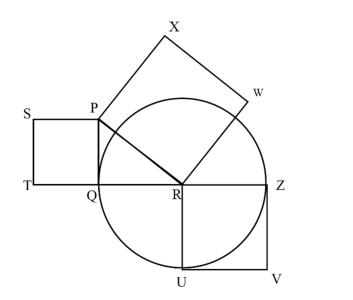
\includegraphics[width=0.5\columnwidth]{figs/q5.png}
\caption{Diagram for Q.5}
\label{fig:q5}
\end{figure}
\begin{multicols}{2}
\begin{enumerate}
    \item Area of SPQT = Area of RUVZ = Area of PXWR
    \item Area of SPQT = Area of PXWR $-$ Area of RUVZ
    \item Area of PXWR = Area of SPQT $-$ Area of RUVZ
    \item Area of PXWR = Area of RUVZ $-$ Area of SPQT
\end{enumerate}
\end{multicols}

\end{enumerate}


\section*{Q.6 -- Q.10 carry two marks each.}

\begin{enumerate}[leftmargin=2.5em, label=\textbf{Q.\arabic*}., itemsep=2em, resume]

\item Healthy eating is a critical component of healthy aging. When should one start eating healthy? It turns out that it is never too early. For example, babies who start eating healthy in the first year are more likely to have better overall health as they get older.  

Which one of the following is the CORRECT logical inference based on the information in the above passage?

\noindent \textbf{[GATE BT 2022]}
\begin{multicols}{2}
\begin{enumerate}
    \item Healthy eating is important for those with good health conditions, but not for others
    \item Eating healthy can be started at any age, earlier the better
    \item Eating healthy and better overall health are more correlated at a young age, but not older age
    \item Healthy eating is more important for adults than kids
\end{enumerate}
\end{multicols}

\item P invested Rs. 5000 per month for 6 months of a year and Q invested Rs. $x$ per month for 8 months of the year in a partnership business. The profit is shared in proportion to the total investment made in that year.  
If at the end of that investment year, Q receives $\dfrac{1}{3}$ of the total profit, what is the value of $x$ (in Rs.)?

\noindent \textbf{[GATE BT 2022]}
\begin{multicols}{2}
\begin{enumerate}
    \item 2500
    \item 3000
    \item 4687
    \item 8437
\end{enumerate}
\end{multicols}

\item The following frequency chart shows the frequency distribution of marks obtained by a set of students in an exam. From the data presented, which one of the following is CORRECT?

\noindent \textbf{[GATE BT 2022]}
\begin{figure}[H]\centering
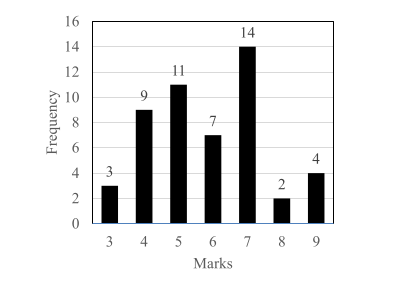
\includegraphics[width=0.6\columnwidth]{figs/q8.png}
\caption{Frequency distribution chart for Q.8}
\label{fig:q8}
\end{figure}
\begin{multicols}{2}
\begin{enumerate}
    \item mean $>$ mode $>$ median
    \item mode $>$ median $>$ mean
    \item mode $>$ mean $>$ median
    \item median $>$ mode $>$ mean
\end{enumerate}
\end{multicols}

\item In the square grid shown, a person standing at P2 is required to move to P5. The only movement allowed for a step involves two moves along one direction followed by one move in a perpendicular direction. The permissible directions for movement are shown as dotted arrows. Without occupying any shaded squares at the end of each step, the minimum number of steps required to go from P2 to P5 is:

\noindent \textbf{[GATE BT 2022]}
\begin{figure}[H]\centering
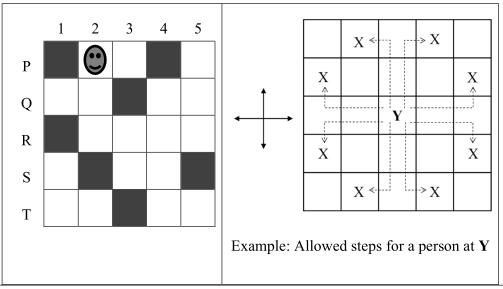
\includegraphics[width=0.6\columnwidth]{figs/q9.png}
\caption{Square grid for Q.9}
\label{fig:q9}
\end{figure}
\begin{multicols}{2}
\begin{enumerate}
    \item 4
    \item 5
    \item 6
    \item 7
\end{enumerate}
\end{multicols}

\item Consider a cube made by folding a single sheet of paper of appropriate shape. The interior faces of the cube are blank. However, the exterior faces that are not visible in the given view may not be blank. Which one of the following represents a possible unfolding of the cube?

\noindent \textbf{[GATE BT 2022]}
\begin{figure}[H]\centering
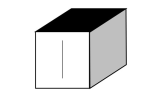
\includegraphics[width=0.6\columnwidth]{figs/q10.png}
\caption{Cube unfolding for Q.10}
\label{fig:q10}
\end{figure}

\begin{figure}[H]\centering
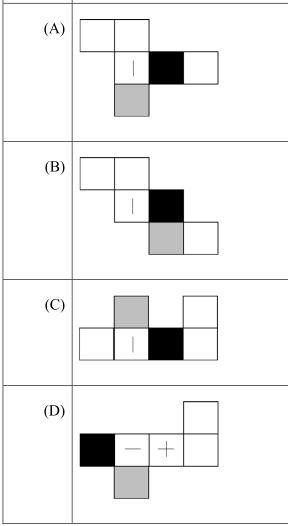
\includegraphics[width=0.6\columnwidth]{figs/q10o.png}
\caption{Options}
\label{fig:q10o}
\end{figure}

\end{enumerate}


\section*{Q.11 -- Q.35 carry one mark each.}

\begin{enumerate}[leftmargin=2.5em, label=\textbf{Q.\arabic*}., itemsep=2em, resume]

\item What is the order of the differential equation given below?
\begin{align*}
x^2 \frac{d^4 y}{dx^4} - 6x^3 \frac{d^2 y}{dx^2} = -2
\end{align*}

\noindent \textbf{[GATE BT 2022]}
\begin{multicols}{2}
\begin{enumerate}
    \item 1
    \item 2
    \item 3
    \item 4
\end{enumerate}
\end{multicols}

\item If the eigenvalues of a $2\times2$ matrix $\mathbf{P}$ are $4$ and $2$, then the eigenvalues of the matrix $\mathbf{P}^{-1}$ are:

\noindent \textbf{[GATE BT 2022]}
\begin{multicols}{2}
\begin{enumerate}
    \item 0, 0
    \item 0.0625, 0.25
    \item 0.25, 0.5
    \item 2, 4
\end{enumerate}
\end{multicols}

\item For a double-pipe heat exchanger, the inside and outside heat transfer coefficients are $100$ and $200~\text{W m}^{-2}\text{K}^{-1}$, respectively. The thickness and thermal conductivity of the thin-walled inner pipe are $1$ cm and $10~\text{W m}^{-1}\text{K}^{-1}$, respectively. The value of the overall heat transfer coefficient is \_\_\_\_\_\_\_ W m$^{-2}$ K$^{-1}$.

\noindent \textbf{[GATE BT 2022]}
\begin{multicols}{2}
\begin{enumerate}
    \item 0.016
    \item 42.5
    \item 62.5
    \item 310
\end{enumerate}
\end{multicols}

\item Match the media component (Column I) with its role (Column II).

\noindent \textbf{[GATE BT 2022]}
\[
\begin{array}{ll}
\text{Column I} & \text{Column II} \\
P. \ \text{Sucrose} & 1. \ \text{Anti-foam agent} \\
Q. \ \text{Zinc chloride} & 2. \ \text{Nitrogen source} \\
R. \ \text{Ammonium sulphate} & 3. \ \text{Carbon source} \\
S. \ \text{Silicone oil} & 4. \ \text{Trace element}
\end{array}
\]
\begin{multicols}{2}
\begin{enumerate}
    \item P-1, Q-2, R-3, S-4
    \item P-2, Q-1, R-3, S-4
    \item P-3, Q-2, R-4, S-1
    \item P-3, Q-4, R-2, S-1
\end{enumerate}
\end{multicols}

\item The binding free energy of a ligand to its receptor protein is $-11.5$ kJ mol$^{-1}$ at 300 K. What is the value of the equilibrium binding constant? Use $R = 8.314$ J mol$^{-1}$ K$^{-1}$.

\noindent \textbf{[GATE BT 2022]}
\begin{multicols}{2}
\begin{enumerate}
    \item 0.01
    \item 1.0
    \item 4.6
    \item 100.5
\end{enumerate}
\end{multicols}

\item The overall stoichiometry for an aerobic cell growth is
\begin{align*}
3C_6H_{12}O_6 + 2.5NH_3 + O_2 \rightarrow 1.5C_aH_bO_cN_d + 3CO_2 + 5H_2O
\end{align*}
What is the elemental composition formula of the biomass?

\noindent \textbf{[GATE BT 2022]}
\begin{multicols}{2}
\begin{enumerate}
    \item C$_9$H$_{18.2}$O$_5$N$_{1.667}$
    \item C$_9$H$_{22.33}$O$_6$N$_{1.667}$
    \item C$_{10}$H$_{18.2}$O$_5$N$_{1.667}$
    \item C$_{10}$H$_{22.33}$O$_6$N$_{1.667}$
\end{enumerate}
\end{multicols}

\item In binomial nomenclature, the name of a bacterial strain is written with the first letter of \_\_\_\_\_ word(s) being capitalized.

\noindent \textbf{[GATE BT 2022]}
\begin{multicols}{2}
\begin{enumerate}
    \item first
    \item second
    \item neither
    \item first and second
\end{enumerate}
\end{multicols}

\item The type of nucleic acid present in $\lambda$-phage is:

\noindent \textbf{[GATE BT 2022]}
\begin{multicols}{2}
\begin{enumerate}
    \item Double stranded DNA
    \item Single stranded circular DNA
    \item Single stranded DNA
    \item Single stranded RNA
\end{enumerate}
\end{multicols}

\item Which of the following statements about reversible enzyme inhibitors are CORRECT?  
P. Uncompetitive inhibitors bind only to the enzyme-substrate complex  
Q. Non-competitive inhibitors bind only at a different site from the substrate  
R. Competitive inhibitors bind to the same site as the substrate

\noindent \textbf{[GATE BT 2022]}
\begin{multicols}{2}
\begin{enumerate}
    \item P and Q only
    \item P and R only
    \item Q and R only
    \item P, Q and R
\end{enumerate}
\end{multicols}

\item Match the component of eukaryotic cells (Column I) with its respective function (Column II).

\noindent \textbf{[GATE BT 2022]}
\[
\begin{array}{ll}
\text{Column I} & \text{Column II} \\
P. \ \text{Lysosome} & 1. \ \text{Digestion of macromolecules} \\
Q. \ \text{Peroxisome} & 2. \ \text{Detoxification of harmful compounds} \\
R. \ \text{Glyoxysome} & 3. \ \text{Conversion of fatty acids to sugar} \\
S. \ \text{Cytoskeleton} & 4. \ \text{Involvement in cell motility}
\end{array}
\]
\begin{multicols}{2}
\begin{enumerate}
    \item P-1, Q-2, R-3, S-4
    \item P-2, Q-1, R-3, S-4
    \item P-3, Q-1, R-2, S-4
    \item P-4, Q-3, R-1, S-2
\end{enumerate}
\end{multicols}

\item In animal cells, the endogenously produced miRNAs silence gene expression by:

\noindent \textbf{[GATE BT 2022]}
\begin{multicols}{2}
\begin{enumerate}
    \item base pairing with the 3$'$-untranslated region of specific mRNAs
    \item blocking mRNA synthesis
    \item binding to the operator site
    \item base pairing with the 3$'$ region of specific rRNAs
\end{enumerate}
\end{multicols}

\item Terpenoids are made of \_\_\_\_\_\_ units.

\noindent \textbf{[GATE BT 2022]}
\begin{multicols}{2}
\begin{enumerate}
    \item amino acid
    \item carbohydrate
    \item isoprene
    \item triacylglycerol
\end{enumerate}
\end{multicols}

\item Match the microbial product (Column I) with its respective application (Column II).

\noindent \textbf{[GATE BT 2022]}
\[
\begin{array}{ll}
\text{Column I} & \text{Column II} \\
P. \ \text{Methane} & 1. \ \text{Biosurfactant} \\
Q. \ \text{Glycolipids} & 2. \ \text{Bioplastic} \\
R. \ \text{Polyhydroxy alkanoate} & 3. \ \text{Biofuel}
\end{array}
\]
\begin{multicols}{2}
\begin{enumerate}
    \item P-1, Q-2, R-3
    \item P-2, Q-1, R-3
    \item P-3, Q-2, R-1
    \item P-3, Q-1, R-2
\end{enumerate}
\end{multicols}

\item Which of the following is NOT used for generating an optimal alignment of two nucleotide sequences?

\noindent \textbf{[GATE BT 2022]}
\begin{multicols}{2}
\begin{enumerate}
    \item Gap penalties
    \item Match scores
    \item Mismatch scores
    \item Nucleotide composition
\end{enumerate}
\end{multicols}

\end{enumerate}

\begin{enumerate}[leftmargin=2.5em, label=\textbf{Q.\arabic*}., itemsep=2em, resume]

\item The recognition sequences of four Type-II restriction enzymes (RE) are given below.  
The symbol (↓) indicates the cleavage site. Identify the RE that generates sticky ends.  

\noindent \textbf{[GATE BT 2022]}
\begin{multicols}{2}
\begin{enumerate}
    \item RE1: 5$'$G↓GATCC3$'$
    \item RE2: 5$'$CTG↓CAG3$'$
    \item RE3: 5$'$CCC↓GGG3$'$
    \item RE4: 5$'$AG↓CT3$'$
\end{enumerate}
\end{multicols}

\item Among individuals in a human population, minor variations exist in nucleotide sequences of chromosomes.  
These variations can lead to gain or loss of sites for specific restriction enzymes.  
Which of the following technique is used to identify such variations?

\noindent \textbf{[GATE BT 2022]}
\begin{multicols}{2}
\begin{enumerate}
    \item Polymerase dependent fragment insertion
    \item Real-time polymerase chain reaction
    \item Restriction fragment length polymorphism
    \item Reverse transcriptase polymerase chain reaction
\end{enumerate}
\end{multicols}

\item Assuming independent assortment and no recombination, the number of different combinations of maternal and paternal chromosomes in gametes of an organism with a diploid number of 12 is \_\_\_\_\_\_\_\_\_.

\noindent \textbf{[GATE BT 2022]}

\item A microorganism is grown in a batch culture using glucose as a carbon source.  
The apparent growth yield is $0.5~\text{g biomass/g substrate}$.  
The initial concentrations of biomass and substrate are $2~\text{g L}^{-1}$ and $200~\text{g L}^{-1}$, respectively.  
Assuming that there is no endogenous metabolism, the maximum biomass concentration that can be achieved is \_\_\_\_\_\_\_\_\_ g L$^{-1}$.

\noindent \textbf{[GATE BT 2022]}

\item The degree of reduction of lactic acid (C$_3$H$_6$O$_3$) is \_\_\_\_\_\_\_\_\_.

\noindent \textbf{[GATE BT 2022]}

\item Consider a nonlinear algebraic equation,
\begin{align*}
x \ln(x) + x - 1 = 0
\end{align*}
Using the Newton-Raphson method, with the initial guess of $x=3$, the value of $x$ after one iteration (rounded off to one decimal place) is \_\_\_\_\_\_\_.

\noindent \textbf{[GATE BT 2022]}

\item The probability density function of a random variable $X$ is
\begin{align*}
p(x) = 2x e^{-x^2}, \quad x \geq 0
\end{align*}
The probability $P(1 \leq X \leq 2)$ (rounded off to two decimal places) is \_\_\_\_\_\_\_.

\noindent \textbf{[GATE BT 2022]}

\item The maximum value of the function
\begin{align*}
f(x) = 3x^2 - x^3, \quad x>0
\end{align*}
is \_\_\_\_\_\_\_.

\noindent \textbf{[GATE BT 2022]}

\item The specific growth rate of a yeast having a doubling time of $0.693$ h (rounded off to nearest integer) is \_\_\_\_\_\_\_ h$^{-1}$.

\noindent \textbf{[GATE BT 2022]}

\item A fermentation broth of density $1000~\text{kg m}^{-3}$ and viscosity $10^{-3}~\text{kg m}^{-1}\text{s}^{-1}$ is mixed in a 100 L fermenter using a $0.1$ m diameter impeller, rotating at a speed of $2~\text{s}^{-1}$.  
The impeller Reynolds number is \_\_\_\_\_\_\_.

\noindent \textbf{[GATE BT 2022]}

\item For a pure species, the slope of the melting line at $-2^{\circ}$C is $-5.0665 \times 10^6~\text{Pa K}^{-1}$.  
The difference between the molar volumes of the liquid and solid phase at $-2^{\circ}$C is $-4.5\times 10^{-6}~\text{m}^3\text{ mol}^{-1}$.  
The value of the latent heat of fusion (rounded off to nearest integer) is \_\_\_\_\_\_\_ J mol$^{-1}$.

\noindent \textbf{[GATE BT 2022]}

\end{enumerate}


\section*{Q.36 -- Q.65 carry two marks each.}

\begin{enumerate}[leftmargin=2.5em, label=\textbf{Q.\arabic*}., itemsep=2em, resume]

\item Which of the following conditions will contribute to the stability of a gene pool in a natural population?  

P. Large population  
Q. No net mutation  
R. Non-random mating  
S. No selection  

\noindent \textbf{[GATE BT 2022]}
\begin{multicols}{2}
\begin{enumerate}
    \item P only
    \item P and Q only
    \item P and R only
    \item P, Q and S only
\end{enumerate}
\end{multicols}

\item Match the media component used in mammalian cell culture (Column I) with its respective role (Column II).

\noindent \textbf{[GATE BT 2022]}
\[
\begin{array}{ll}
\text{Column I} & \text{Column II} \\
P. \ \text{Hydrocortisone} & 1. \ \text{Mitogen} \\
Q. \ \text{Fibronectin} & 2. \ \text{Vitamin} \\
R. \ \text{Epidermal growth factor} & 3. \ \text{Hormone} \\
S. \ \text{Riboflavin} & 4. \ \text{Cell attachment}
\end{array}
\]
\begin{multicols}{2}
\begin{enumerate}
    \item P-3, Q-4, R-1, S-2
    \item P-3, Q-4, R-2, S-1
    \item P-4, Q-3, R-1, S-2
    \item P-4, Q-3, R-2, S-1
\end{enumerate}
\end{multicols}

\item Match the cell type (Column I) with its function (Column II).

\noindent \textbf{[GATE BT 2022]}
\[
\begin{array}{ll}
\text{Column I} & \text{Column II} \\
P. \ \text{B cells} & 1. \ \text{Humoral immunity} \\
Q. \ \text{Neutrophils} & 2. \ \text{Cytotoxicity} \\
R. \ \text{T cells} & 3. \ \text{Histamine-associated allergy} \\
S. \ \text{Mast cells} & 4. \ \text{Phagocytosis}
\end{array}
\]
\begin{multicols}{2}
\begin{enumerate}
    \item P-1, Q-2, R-3, S-4
    \item P-1, Q-4, R-2, S-3
    \item P-4, Q-3, R-1, S-2
    \item P-4, Q-3, R-2, S-1
\end{enumerate}
\end{multicols}

\item A $2\times2$ matrix $\mathbf{P}$ has an eigenvalue $\lambda=2$ with eigenvector $\myvec{1\\0}$ and another eigenvalue $\lambda=5$, with eigenvector $\myvec{1\\1}$. The matrix $\mathbf{P}$ is:

\noindent \textbf{[GATE BT 2022]}
\begin{multicols}{2}
\begin{enumerate}
    \item $\myvec{2 & 0 \\ 0 & 5}$
    \item $\myvec{2 & 3 \\ 0 & 5}$
    \item $\myvec{1 & 1 \\ 0 & 1}$
    \item $\myvec{1 & 1 \\ 1 & 0}$
\end{enumerate}
\end{multicols}

\item Match the stationary phase (Column I) with its corresponding chromatography technique (Column II).

\noindent \textbf{[GATE BT 2022]}
\[
\begin{array}{ll}
\text{Column I} & \text{Column II} \\
P. \ \text{Protein A} & 1. \ \text{Size exclusion chromatography} \\
Q. \ \text{Sephadex} & 2. \ \text{Ion-exchange chromatography} \\
R. \ \text{Phenylsepharose} & 3. \ \text{Affinity chromatography} \\
S. \ \text{Diethylaminoethyl cellulose} & 4. \ \text{Hydrophobic interaction chromatography}
\end{array}
\]
\begin{multicols}{2}
\begin{enumerate}
    \item P-1, Q-4, R-2, S-3
    \item P-3, Q-1, R-4, S-2
    \item P-3, Q-4, R-2, S-1
    \item P-4, Q-1, R-3, S-2
\end{enumerate}
\end{multicols}

\item Which of the following statements are CORRECT for a controller?  

P. In a proportional controller, a control action is proportional to the error  
Q. In an integral controller, a control action is proportional to the derivative of the error  
R. There is no ``offset'' in the response of the closed-loop first-order process with a proportional controller  
S. There is no ``offset'' in the response of the closed-loop first-order process with a proportional-integral controller  

\noindent \textbf{[GATE BT 2022]}
\begin{multicols}{2}
\begin{enumerate}
    \item P and Q only
    \item P and R only
    \item P and S only
    \item Q and S only
\end{enumerate}
\end{multicols}

\item Which of the following are CORRECT about protein structure?  

P. Secondary structure is formed by a repeating pattern of interactions among the polypeptide backbone atoms  
Q. Tertiary structure is the three-dimensional arrangement of the polypeptide backbone atoms only  
R. Quaternary structure refers to an assembly of multiple polypeptide subunits  

\noindent \textbf{[GATE BT 2022]}
\begin{multicols}{2}
\begin{enumerate}
    \item P and Q only
    \item P and R only
    \item Q and R only
    \item P, Q and R
\end{enumerate}
\end{multicols}

\item The enzymes involved in ubiquitinylation of cell-cycle proteins are:

\noindent \textbf{[GATE BT 2022]}
\begin{multicols}{2}
\begin{enumerate}
    \item E1 and E2 only
    \item E1 and E3 only
    \item E1 and E4 only
    \item E1, E2 and E3
\end{enumerate}
\end{multicols}

\item The maximum parsimony method is used to construct a phylogenetic tree for a set of sequences.  
Which one of the following statements about the method is CORRECT?

\noindent \textbf{[GATE BT 2022]}
\begin{multicols}{2}
\begin{enumerate}
    \item It predicts the tree that minimizes the steps required to generate the observed variations
    \item It predicts the tree that maximizes the steps required to generate the observed variations
    \item It predicts the tree with the least number of branch points
    \item It employs probability calculations to identify the tree
\end{enumerate}
\end{multicols}

\item Which of the following spectroscopic technique(s) can be used to identify all the functional groups of an antibiotic contaminant in food?  

P. Infrared  
Q. Circular dichroism  
R. Nuclear magnetic resonance  
S. UV-Visible  

\noindent \textbf{[GATE BT 2022]}
\begin{multicols}{2}
\begin{enumerate}
    \item P only
    \item P and R only
    \item P, Q and R only
    \item P, Q, R and S
\end{enumerate}
\end{multicols}

\end{enumerate}

\begin{enumerate}[leftmargin=2.5em, label=\textbf{Q.\arabic*}., itemsep=2em, resume]

\item Adenine can undergo a spontaneous change to hypoxanthine in a cell, leading to a DNA base pair mismatch.  
The CORRECT combination of enzymes that are involved in repairing this damage is:

\noindent \textbf{[GATE BT 2022]}

\begin{multicols}{2}
\begin{enumerate}
    \item Nuclease, DNA polymerase, DNA ligase
    \item Nuclease, DNA ligase, helicase
    \item Primase, DNA polymerase, DNA ligase
    \item Primase, helicase, DNA polymerase
\end{enumerate}
\end{multicols}

\item Consider the ordinary differential equation
\begin{align*}
\frac{dy}{dx} = f(x,y) = 2x - y^2
\end{align*}
If $y(1) = 1$, the value(s) of $y(1.5)$ using Euler’s implicit method
\[
y_{n+1} = y_n + h f(x_{n+1}, y_{n+1})
\]
with a step size $h=0.5$, is (are):

\noindent \textbf{[GATE BT 2022]}

\begin{multicols}{2}
\begin{enumerate}
    \item $-1 - 5\sqrt{0.3}$
    \item $-1 + 5\sqrt{0.3}$
    \item $1 + 5\sqrt{0.3}$
    \item $1 - 5\sqrt{0.3}$
\end{enumerate}
\end{multicols}

\item Which of the following statements are CORRECT for an enzyme entrapped in a spherical particle?

\noindent \textbf{[GATE BT 2022]}
\begin{multicols}{2}
\begin{enumerate}
    \item Effectiveness factor is ratio of the reaction rate with diffusion-limitation to the reaction rate without diffusion-limitation
    \item Internal diffusion is rate-limiting at low values of Thiele modulus
    \item Effectiveness factor increases with decrease in Thiele modulus
    \item Internal diffusion-limitation can be reduced by decreasing the size of the particle
\end{enumerate}
\end{multicols}

\item Which of the following is(are) COMMON feature(s) for both aerobic and anaerobic bacterial cultures?

\noindent \textbf{[GATE BT 2022]}
\begin{multicols}{2}
\begin{enumerate}
    \item Glycolysis
    \item NAD$^+$ is the oxidising agent
    \item Oxidative phosphorylation
    \item Two net ATP molecules formed per glucose molecule
\end{enumerate}
\end{multicols}

\item Which of the following plot(s) is(are) CORRECT for an enzyme that obeys Michaelis-Menten kinetics, assuming $[S] \ll K_M$?  
Here $[S]$ is the concentration of the substrate, $K_M$ is the Michaelis constant, and $v_0$ is the initial reaction velocity.

\noindent \textbf{[GATE BT 2022]}
\begin{figure}[H]\centering
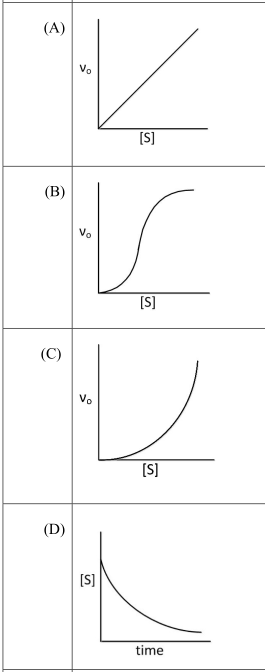
\includegraphics[width=0.6\columnwidth]{figs/q50.png}
\caption{Plots for Q.50}
\label{fig:q50}
\end{figure}

\item Which of the following statement(s) is(are) CORRECT regarding the lac operon in \textit{E. coli} when grown in the presence of glucose and lactose?

\noindent \textbf{[GATE BT 2022]}
\begin{multicols}{2}
\begin{enumerate}
    \item At low glucose level, the operon is activated
    \item At high glucose level, the operon is activated to enable the utilization of lactose
    \item The lac repressor binds to operator region inactivating the operon
    \item Binding of lactose to the lac repressor induces the operon
\end{enumerate}
\end{multicols}

\item Emerging viruses such as SARS-CoV2 cause epidemics. Which of the following process(es) contribute to the rise of such viruses?

\noindent \textbf{[GATE BT 2022]}
\begin{multicols}{2}
\begin{enumerate}
    \item Mutation of existing virus
    \item Jumping of existing virus from current to new hosts
    \item Spread of virus in the new host population
    \item Replication of virus outside a host
\end{enumerate}
\end{multicols}

\item Introduction of foreign genes into plant cells can be carried out using:

\noindent \textbf{[GATE BT 2022]}
\begin{multicols}{2}
\begin{enumerate}
    \item Agrobacterium
    \item CaCl$_2$ mediated plasmid uptake
    \item Electroporation
    \item Gene gun
\end{enumerate}
\end{multicols}

\item Which of the following statement(s) regarding trafficking in eukaryotic cells is(are) CORRECT?

\noindent \textbf{[GATE BT 2022]}
\begin{multicols}{2}
\begin{enumerate}
    \item Dynamin binds GTP and is involved in vesicle budding
    \item Dynamin is involved in cytoskeletal remodelling
    \item Dynein binds ATP and is involved in movement of organelles along microtubules
    \item Dynein binds GTP and is involved in movement of organelles along microtubules
\end{enumerate}
\end{multicols}

\item Consider a random variable $X$ with mean $\mu = 0.1$ and variance $\sigma^2 = 0.2$.  
A new random variable $Y = 2X + 1$ is defined.  
The variance of $Y$ (rounded off to one decimal place) is \_\_\_\_\_\_\_.

\noindent \textbf{[GATE BT 2022]}

\item For $x_1 > 0$ and $x_2 > 0$, the value of
\begin{align*}
\lim_{x_1 \to x_2} \frac{\ln(x_1) - \ln(x_2)}{x_1 - x_2}
\end{align*}
is \_\_\_\_\_\_\_.

\noindent \textbf{[GATE BT 2022]}

\item Figure below depicts simplified metabolic and transport reactions taking place in the production of B from A in a cell.  
The subscript ‘i’ refers to intracellular metabolites.  
$r_j$ is the $j^{th}$ reaction flux. Under pseudo-steady-state condition, the following reaction fluxes are available: $r_1=4$, $r_3=1$, $r_6=1$.  
The transport flux of B, $r_4$, is \_\_\_\_\_\_\_.

\noindent \textbf{[GATE BT 2022]}
\begin{figure}[H]\centering
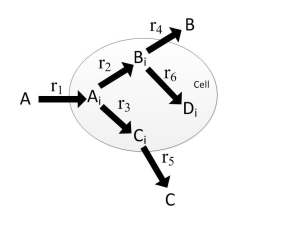
\includegraphics[width=0.6\columnwidth]{figs/q57.png}
\caption{Metabolic network for Q.57}
\label{fig:q57}
\end{figure}

\item The amount of biomass in a reactor at the end of the batch process is 50 g.  
Fed-batch operation is initiated by feeding the substrate solution at a constant rate of 1 L h$^{-1}$.  
The concentration of substrate in the feed is 50 g L$^{-1}$.  
The maximum biomass yield $Y_{x/s}$ is 0.4 g/g.  
Assuming the system is at quasi-steady state, the maximum amount of biomass after 5 h of feeding is \_\_\_\_\_\_\_ g.

\noindent \textbf{[GATE BT 2022]}

\item An enzyme catalyzes the conversion of substrate A into product B.  
The rate equation for this reaction is
\[
-r_A = \frac{5C_A}{1 + C_A}, \quad \text{mol L}^{-1}\text{min}^{-1}
\]
Substrate A at an initial concentration of 10 mol L$^{-1}$ enters an ideal mixed flow reactor (MFR) at a flow rate of 10 L min$^{-1}$.  
The volume of the MFR required for 50\% conversion of substrate to product is \_\_\_\_\_\_\_ L.

\noindent \textbf{[GATE BT 2022]}

\item Liquid-phase mass transfer coefficient ($k_L$) is measured in a stirred tank vessel using steady-state method by sparging air.  
Oxygen uptake by the microorganism is measured.  
The bulk concentration of O$_2$ is $10^{-4}$ mol L$^{-1}$.  
Solubility of O$_2$ in water at 25$^{\circ}$C is $10^{-3}$ mol L$^{-1}$.  
If the oxygen consumption rate is $9\times10^{-4}$ mol L$^{-1}$ s$^{-1}$, and interfacial area is $100~\text{m}^2/\text{m}^3$, the value of $k_L$ is \_\_\_\_\_\_\_ cm s$^{-1}$.

\noindent \textbf{[GATE BT 2022]}

\item Consider a piston-cylinder assembly shown in the figure below.  
The walls of the cylinder are insulated. The cylinder contains 1 mole of an ideal gas at 300 K and the piston is held initially at position $z_1$ using a stopper.  
After the stopper is removed, the piston suddenly rises against atmospheric pressure $(1.013 \times 10^5$ Pa) to the new position $z_2$ where it is held by another stopper.  
The heat capacity ($C_v$) of the gas is 12.5 J mol$^{-1}$ K$^{-1}$.  
The cross-sectional area of the cylinder is $10^{-3}$ m$^2$.  
Assume the piston is weightless and frictionless.  
If $z_2 - z_1 = 1$ m, the final temperature of the gas (rounded off to nearest integer) is \_\_\_\_\_\_\_ K.

\noindent \textbf{[GATE BT 2022]}
\begin{figure}[H]\centering
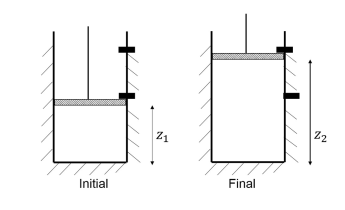
\includegraphics[width=0.6\columnwidth]{figs/q61.png}
\caption{Piston-cylinder assembly for Q.61}
\label{fig:q61}
\end{figure}

\item Consider the growth of \textit{S. cerevisiae} under aerobic condition in a bioreactor and the specific growth rate of yeast is $0.5$ h$^{-1}$.  
The overall reaction of the process is  
\[
2C_6H_{12}O_6 + 0.2NH_3 + 10.35O_2 \rightarrow CH_{1.8}O_{0.5}N_{0.2} + 0.2C_2H_6O + 10.6CO_2 + 10.8H_2O
\]
The heat of combustion values for different compounds are tabulated (reference: CO$_2$, H$_2$O, O$_2$, N$_2$ at standard conditions).  
The specific rate of heat production (rounded off to nearest integer) is \_\_\_\_\_\_\_ kJ mol$^{-1}$ h$^{-1}$.

\noindent \textbf{[GATE BT 2022]}

\item A pilot sterilization was carried out in a vessel containing 100 m$^3$ medium with an initial spore concentration of $10^8$ spores/ml.  
The accepted level of contamination after sterilization is 1 spore in the entire vessel.  
The specific death rate constant for the spore is $2$ min$^{-1}$ at 121$^\circ$C.  
Assuming no death takes place during the heating and cooling cycles, the holding time at 121$^\circ$C (rounded off to nearest integer) is \_\_\_\_\_\_\_ min.

\noindent \textbf{[GATE BT 2022]}

\item A circular plasmid has three different but unique restriction sites for enzymes ‘a’, ‘b’ and ‘c’.  
When enzymes ‘a’ and ‘b’ are used together, two fragments of equal size are generated.  
Enzyme ‘c’ creates fragments of equal size only from one of the fragments generated by those cleaved by ‘a’ and ‘b’.  
The plasmid is treated with a mixture of ‘a’, ‘b’ and ‘c’ and analysed by agarose gel electrophoresis.  
The number of bands observed in the gel is \_\_\_\_\_\_\_.

\noindent \textbf{[GATE BT 2022]}

\item A bacterial strain is grown in nutrient medium at 37$^\circ$C under aerobic conditions.  
The medium is inoculated with $10^2$ cells from a seed culture.  
If the number of cells in the culture is $10^5$ after 10 hours of growth, the doubling time of the strain (rounded off to nearest integer) is \_\_\_\_\_\_\_ h.

\noindent \textbf{[GATE BT 2022]}

\end{enumerate}

\end{document}